\documentclass[manuscript,screen]{../acmart}
\geometry{paperwidth=15cm,paperheight=8cm,margin=4mm}
\setcopyright{none}
\usepackage{tikz}
\usetikzlibrary{arrows.meta,positioning,fit,backgrounds}
\pagestyle{empty}
\begin{document}
\pagestyle{empty}\thispagestyle{empty}
\noindent
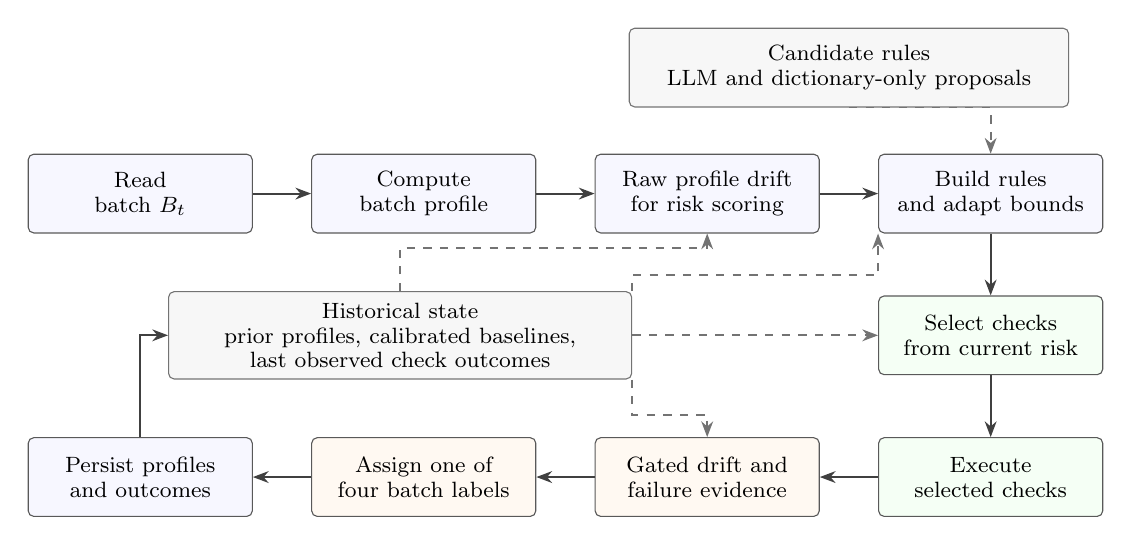
\begin{tikzpicture}[
  x=1cm,y=1cm,
  box/.style={draw=black!65,rounded corners=2pt,align=center,
    font=\fontsize{8}{9}\selectfont,minimum height=10mm,text width=26mm,
    inner sep=3.5pt,fill=blue!3},
  store/.style={draw=black!55,rounded corners=2pt,align=center,
    font=\fontsize{8}{9}\selectfont,minimum height=10mm,inner sep=4pt,fill=black!3},
  arr/.style={-{Stealth[length=2mm]},line width=.7pt,draw=black!75},
  state/.style={arr,dashed,draw=black!55}]
\node[box] (read) at (0,0) {Read\\batch $B_t$};
\node[box] (prof) at (3.6,0) {Compute\\batch profile};
\node[box] (raw) at (7.2,0) {Raw profile drift\\for risk scoring};
\node[box] (build) at (10.8,0) {Build rules\\and adapt bounds};
\node[box,fill=green!4] (select) at (10.8,-1.8) {Select checks\\from current risk};
\node[box,fill=green!4] (execute) at (10.8,-3.6) {Execute\\selected checks};
\node[box,fill=orange!5] (gate) at (7.2,-3.6) {Gated drift and\\failure evidence};
\node[box,fill=orange!5] (label) at (3.6,-3.6) {Assign one of\\four batch labels};
\node[box] (persist) at (0,-3.6) {Persist profiles\\and outcomes};
\node[store,text width=56mm] (history) at (3.3,-1.8)
  {Historical state\\prior profiles, calibrated baselines,\\last observed check outcomes};
\node[store,text width=53mm] (candidates) at (9.0,1.6)
  {Candidate rules\\LLM and dictionary-only proposals};
\draw[arr] (read)--(prof);
\draw[arr] (prof)--(raw);
\draw[arr] (raw)--(build);
\draw[arr] (build)--(select);
\draw[arr] (select)--(execute);
\draw[arr] (execute)--(gate);
\draw[arr] (gate)--(label);
\draw[arr] (label)--(persist);
\draw[arr] (persist.north) |- (history.west);
\draw[state] (candidates.south) -| (build.north);
\draw[state] (history.north) -- ++(0,.55) -| (raw.south);
\draw[state] (history.east) -- (select.west);
\draw[state] (history.south east) -- ++(0,-.45) -| (gate.north);
\draw[state] (history.north east) -- ++(0,.20) -| (build.south west);
\end{tikzpicture}
\end{document}


